\documentclass{scrartcl} 
\usepackage[ngerman,english]{babel}
 \usepackage[T1]{fontenc}
\usepackage{lmodern}
\usepackage[applemac]{inputenc}

\usepackage{amsmath}
\usepackage{amssymb}
\usepackage{amstext}
\usepackage{amsthm}

\usepackage{fancyhdr}
\usepackage{paralist}

\usepackage{mathtools}


\usepackage{hyperref}

\DeclareMathOperator*{\esssup}{ess.sup}
\DeclareMathOperator*{\defgl}{\vcentcolon=}


%\pagestyle{fancy}
%\fancyhead[L]{Seminar \glqq Optimale Steuerung\grqq\\ Prof. Brokate, Prof. Kuttler} %Kopfzeile links
%\fancyhead[C]{} %zentrierte Kopfzeile
%\fancyhead[R]{10. Dezember 2013\\ Manuel Demmeler} %Kopfzeile rechts
\title{\vspace{-1.3cm} \textmd{\normalsize{Project description}}\\ Parallelization of the PRM Method}
\date{}
\author{Manuel Demmeler}

%\thispagestyle{fancy}

\newcommand{\3}{ ^{3\times3} }
\newcommand{\R}{\mathbb{R}}
\newcommand{\N}{\mathbb{N}}
\newcommand{\M}{\mathbb{M}}
\newcommand{\Sym}{\mathbb{S}^3}
\newcommand{\Mpos}{\M_+^3}
\newcommand{\Orth}{\mathbb{O}^3}
\newcommand{\norm}[1]{\left\lVert#1\right\rVert}
\newcommand{\abs}[1]{\left |#1\right |}
\newcommand{\ub}{\bar{u}}
\newcommand{\yb}{\bar{y}}
\newcommand{\scprod}[2]{\langle#1 , #2 \rangle}

%\vspace{-3.4cm}


\begin{document}
\maketitle

\section{Motivation}
In trajctory optimization with obstacles, it is often necessary to provide feasible inital trajectories. 
For example in robot motion planning, where the dimensions of the underlying spaces are rather high, this can be expensive. A further problem is that because of the transformation from work into configuration space, the obstacles are often no longer given in a closed form. An efficient approximative approach is using probabilistic roadmaps (PRMs).



\section{Problem Statement and Sequential PRM Method}
\newtheorem*{defi}{Definition}
\newtheorem*{alg1}{Algorithm}


The abstract problem is to find a path on a d-dimensional map, which avoids intersecting obstacles. The obstacles are  given by an indicator function
\begin{equation*}
	I: \Omega \rightarrow \{0, 1\}
\end{equation*}
on the domain \( \Omega = [ q_{min,1}, q_{max,1} ] \times ... \times  [ q_{min,d}, q_{max,d} ] \subset \R^d  \) and the goal is to find a continuous way
\begin{equation*}
	\Gamma: [0,1] \rightarrow \Omega
\end{equation*}
between a given start and endpoint, \(\Gamma(0)=q_b,\ \Gamma(1)=q_e \), 
such that
\begin{equation*}
	I(\Gamma(s))=0 \text{\ f.a.\ } s�\in [0,1].
\end{equation*}
The probabilistic roadmap (PRM) approach grows a graph \(G=(V,E)\) form \(q_s\) and \(q_e\) by randomly sampling nodes \(v\in V\subset \Omega\).  Two nodes \(v,w \in V\) are connected, if they are near enough each other and the linear connection in between is free from obstacles. The algorithm terminates, when there is a path from \(q_s\) to \(q_e\) on G.
\begin{defi}
For two points \(q_1\) and \(q_2\) we define the connection with stepsize \(h>0\) as
	\begin{equation*}
		[q_1,q_2]_h \defgl \{ q = \lambda q_1+(1-\lambda) q_2\ |\ \lambda \in [0,1], \norm{q-q_1} \in \N_0 h \}.
	\end{equation*}
	We say, \(q_1\) and \(q_2\) are connected (with stepsize \(h>0\)) on the map \(\Omega\), if
	\(I(q)=0\) for all \(q \in [q_1, q_2]_h\).
\end{defi}
\begin{alg1} (Probabilistic Roadmap in general)\\
	Input: \(q_s, q_e\in \Omega, h>0, d_0>0\)	\\
	Output: \(q_s=q_1, ... ,q_n=q_e\in \Omega\), 
		such that all \(q_i\) and \(q_{i+1}\) are connected with stepsize \(h\)
	\begin{itemize}
		\item Initialize graph \(G=(V,E)\) with \(V=\{q_s, q_e\}\), 
			if \(q_s\) and \(q_e\) are connected, \(E \leftarrow\{ q_s, q_e\}\)
		\item While there exists no path in G between \(q_s\) and \(q_e\) do
		\begin{itemize}
			\item Sample \(q\in \Omega\) from a probability density  \(p(\ \cdot\ , G)\), resample until \(I(q)=0\)
			\item \(V \leftarrow{q}\)
			\item For all nodes \(\tilde{q} \in V\) which are near enough (\( \norm{q- \tilde q} \le d_0 \)) and
				connected with \(q\) with stepsize h, 
				\(E \leftarrow \{q, \tilde{q}\}\)
		\end{itemize}
		\item Determine the shortest path \(q_1, ... , q_n\in V\) on \(G\) from \(q_s\) to \(q_e\).
	\end{itemize}
\end{alg1}


The probability density \(p(\ \cdot\ ,G)\) (depending on the actual graph) can be for example first select randomly a node \(q_0 \in V\) and then sample a new node \(q\) in the neighbourhood of \(q_0\). Theory about success probabilities and convergence results can be found in \cite{prmlec}, \cite{prm1} or \cite{prm2}.


\section{Application to Robotics}

In the project, it is planned to use this algorithm to create collisionfree trajectories of a robot arm. 
For a robot with d joint angles \(q_i\) one can calculate straightforwardly all positions \(x_j \in \R^3\) and orientations \(R_j\in \R^{3\times3}\) of the single parts of the robot. Therefore the direct kinematic can be interpreted as a (strongly nonlinear) function
\begin{equation*}
	f: (q_1, ... , q_d) \mapsto (x_1, R_1, ..., x_l, R_l).
\end{equation*}

Now, we have given some obstacles with fixed positions \(x_{l+1}, ..., x_m\) and orientations \(R_{l+1}, ..., R_{m}\), which the robot has to avoid during movement. It is assumed that all objects are given in a form, that for each two objects it can be determined from the positions and orientations, if there is an intersection. For example as polyhedrons.
From this the indicator function can be defined as
\begin{equation*}
	I(q)=
	\begin{cases}
		0,	& \text{if no collision for all object pairs\ } (x_j, R_j), (x_k,R_k),\ j,k\in 1, ... , m \\
		1,	& \text{for at least one collision}
	\end{cases}
\end{equation*}
Now, if we additionally introduce jointlimits and call the set of possible angles \(\Omega\), we see, that the problem of finding feasible trajectories is exactly the pathfinding problem from above. 

It has to be noted that the trajectories \(q(t)\) the PRM algorithm generates are piecewise linear and therefore not differentiable. Hence, they have to be smoothed before the use on a robot. This is expectedly not part of the project.

\begin{figure}
    \centering
    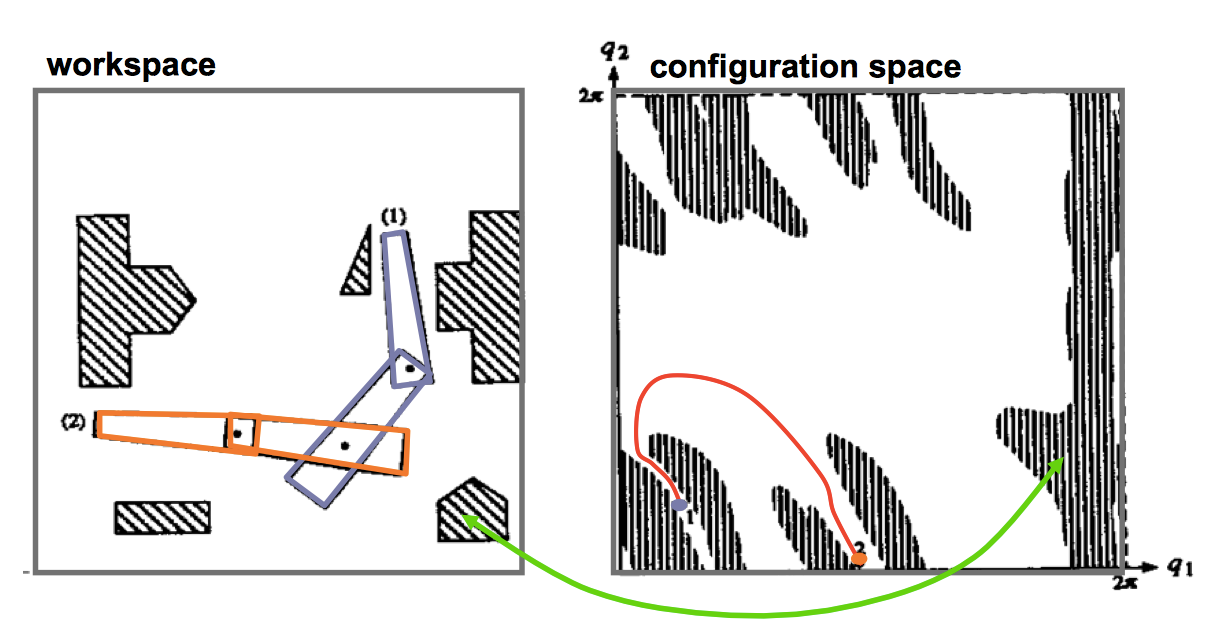
\includegraphics[width=0.8\textwidth]{configspacetrafo.png}
    \caption{Example for the transformation of obstacles into configspace. 
    		The scattered areas on the right are the sets of points with I(q)=1, \cite{prmlec}.}
    \label{fig:awesome_image}
\end{figure}


\section{Ideas for Parallelization}

Like the stated robotics example, in many cases the most costly operation of the PRM algorithm is the evaluation of the indicator function \(I(q)\), which however can be done independently for every new \(q\).
\begin{itemize}
\item 
Therefore in a first step, it is planned to implement \(I(q)\) parallely in a vectorized way, i.e. as a function \((q_1, ... , q_P) \mapsto (I(q_1),...,I(q_P))\). For example with help of the GPU. In the robotics example this means, the direct kinematic and collision calculation is made parallely for \(P\) different joint angle values.
\item
Then in a first level of parallelization, this function can be applied to the \(q_i \in [q, \tilde q]_h \) to check, if \(q\) and \(\tilde q\) are connected.
\item
Furthermore, a second level of parallelization could be achieved by sampling and connecting several new points \(\tilde q_i\) parallely. This is expected to be more difficult, because all new nodes have to be connected to the old graph and to each other. Therefore it has to be evaluated, if a parallel implementation stays efficient here.
\item
If there remains time, a next idea could be to execute the algorithm on different discretization levels \(h\). This means for example to compute a way \(q_1^0, ..., q_n^0\) which is connected with a coarse stepsize \(h_0\), then to decrease the stepsize to \(0<h_1<h_0\) and take the path nodes \(q_i^0\) as starting nodes for the next execution of the algorithm, which gives then an \(h_1\)-connected way \(q_1^1, ... , q_n^1\), etc.
\end{itemize}



\bibliographystyle{alpha}
\begin{thebibliography}{999}
	\bibitem{prmlec} D. Burschka, Lecture Robot Motion Planning, source: http://robvis01.informatik.tu-muenchen.de/courses/wegtraj/index.html
	\bibitem{prm1} H. Choset, K. Lynch, S. Hutchinson, G. Kantor, W. Burgard, L. Kavraki and S. Thrun, Principles of Robot Motion: Theory, Algorithms, and Implementation, MIT Press, 2005
	\bibitem{prm2} S. M. LaValle, Planning Algorithms, Cambridge University Press, 2006
	\bibitem{robodyn} T. Buschmann, Skript zur Vorlesung: Roboterdynamik SS14, Lehrstuhl f�r Angewandte Mechanik, TU M�nchen, 2014
\end{thebibliography}

\end{document}


















